%%%%%%%%%%%%%%%%%%%%%%%%%%%%%%%%%%%%%%%%%
% Lachaise Assignment
% LaTeX Template
% Version 1.0 (26/6/2018)
%
% This template originates from:
% http://www.LaTeXTemplates.com
%
% Authors:
% Marion Lachaise & François Févotte
% Vel (vel@LaTeXTemplates.com)
%
% License:
% CC BY-NC-SA 3.0 (http://creativecommons.org/licenses/by-nc-sa/3.0/)
% 
%%%%%%%%%%%%%%%%%%%%%%%%%%%%%%%%%%%%%%%%%

%----------------------------------------------------------------------------------------
%	PACKAGES AND OTHER DOCUMENT CONFIGURATIONS
%----------------------------------------------------------------------------------------
\documentclass{article}
\usepackage{hyperref}
\usepackage{wrapfig}
\usepackage[spanish]{babel}

\renewcommand{\spanishtablename}{Tabla}

%%%%%%%%%%%%%%%%%%%%%%%%%%%%%%%%%%%%%%%%%
% Lachaise Assignment
% Structure Specification File
% Version 1.0 (26/6/2018)
%
% This template originates from:
% http://www.LaTeXTemplates.com
%
% Authors:
% Marion Lachaise & François Févotte
% Vel (vel@LaTeXTemplates.com)
%
% License:
% CC BY-NC-SA 3.0 (http://creativecommons.org/licenses/by-nc-sa/3.0/)
% 
%%%%%%%%%%%%%%%%%%%%%%%%%%%%%%%%%%%%%%%%%

%----------------------------------------------------------------------------------------
%	PACKAGES AND OTHER DOCUMENT CONFIGURATIONS
%----------------------------------------------------------------------------------------

\usepackage{amsmath,amsfonts,stmaryrd,amssymb} % Math packages

\usepackage{enumerate} % Custom item numbers for enumerations

\usepackage[ruled]{algorithm2e} % Algorithms

\usepackage[framemethod=tikz]{mdframed} % Allows defining custom boxed/framed environments

\usepackage{listings} % File listings, with syntax highlighting
\lstset{
	basicstyle=\ttfamily, % Typeset listings in monospace font
}

%----------------------------------------------------------------------------------------
%	DOCUMENT MARGINS
%----------------------------------------------------------------------------------------

\usepackage{geometry} % Required for adjusting page dimensions and margins

\geometry{
	paper=a4paper, % Paper size, change to letterpaper for US letter size
	top=2.5cm, % Top margin
	bottom=3cm, % Bottom margin
	left=2.5cm, % Left margin
	right=2.5cm, % Right margin
	headheight=14pt, % Header height
	footskip=1.5cm, % Space from the bottom margin to the baseline of the footer
	headsep=1.2cm, % Space from the top margin to the baseline of the header
	%showframe, % Uncomment to show how the type block is set on the page
}

%----------------------------------------------------------------------------------------
%	FONTS
%----------------------------------------------------------------------------------------

\usepackage[utf8]{inputenc} % Required for inputting international characters
\usepackage[T1]{fontenc} % Output font encoding for international characters

\usepackage{XCharter} % Use the XCharter fonts

%----------------------------------------------------------------------------------------
%	COMMAND LINE ENVIRONMENT
%----------------------------------------------------------------------------------------

% Usage:
% \begin{commandline}
%	\begin{verbatim}
%		$ ls
%		
%		Applications	Desktop	...
%	\end{verbatim}
% \end{commandline}

\mdfdefinestyle{commandline}{
	leftmargin=10pt,
	rightmargin=10pt,
	innerleftmargin=15pt,
	middlelinecolor=black!50!white,
	middlelinewidth=2pt,
	frametitlerule=false,
	backgroundcolor=black!5!white,
	frametitle={Command Line},
	frametitlefont={\normalfont\sffamily\color{white}\hspace{-1em}},
	frametitlebackgroundcolor=black!50!white,
	nobreak,
}

% Define a custom environment for command-line snapshots
\newenvironment{commandline}{
	\medskip
	\begin{mdframed}[style=commandline]
}{
	\end{mdframed}
	\medskip
}

%----------------------------------------------------------------------------------------
%	FILE CONTENTS ENVIRONMENT
%----------------------------------------------------------------------------------------

% Usage:
% \begin{file}[optional filename, defaults to "File"]
%	File contents, for example, with a listings environment
% \end{file}

\mdfdefinestyle{file}{
	innertopmargin=1.6\baselineskip,
	innerbottommargin=0.8\baselineskip,
	topline=false, bottomline=false,
	leftline=false, rightline=false,
	leftmargin=2cm,
	rightmargin=2cm,
	singleextra={%
		\draw[fill=black!10!white](P)++(0,-1.2em)rectangle(P-|O);
		\node[anchor=north west]
		at(P-|O){\ttfamily\mdfilename};
		%
		\def\l{3em}
		\draw(O-|P)++(-\l,0)--++(\l,\l)--(P)--(P-|O)--(O)--cycle;
		\draw(O-|P)++(-\l,0)--++(0,\l)--++(\l,0);
	},
	nobreak,
}

% Define a custom environment for file contents
\newenvironment{file}[1][File]{ % Set the default filename to "File"
	\medskip
	\newcommand{\mdfilename}{#1}
	\begin{mdframed}[style=file]
}{
	\end{mdframed}
	\medskip
}

%----------------------------------------------------------------------------------------
%	NUMBERED QUESTIONS ENVIRONMENT
%----------------------------------------------------------------------------------------

% Usage:
% \begin{question}[optional title]
%	Question contents
% \end{question}

\mdfdefinestyle{question}{
	innertopmargin=1.2\baselineskip,
	innerbottommargin=0.8\baselineskip,
	roundcorner=5pt,
	nobreak,
	singleextra={%
		\draw(P-|O)node[xshift=1em,anchor=west,fill=white,draw,rounded corners=5pt]{%
		Question \theQuestion\questionTitle};
	},
}

\newcounter{Question} % Stores the current question number that gets iterated with each new question

% Define a custom environment for numbered questions
\newenvironment{question}[1][\unskip]{
	\bigskip
	\stepcounter{Question}
	\newcommand{\questionTitle}{~#1}
	\begin{mdframed}[style=question]
}{
	\end{mdframed}
	\medskip
}

%----------------------------------------------------------------------------------------
%	WARNING TEXT ENVIRONMENT
%----------------------------------------------------------------------------------------

% Usage:
% \begin{warn}[optional title, defaults to "Warning:"]
%	Contents
% \end{warn}

\mdfdefinestyle{warning}{
	topline=false, bottomline=false,
	leftline=false, rightline=false,
	nobreak,
	singleextra={%
		\draw(P-|O)++(-0.5em,0)node(tmp1){};
		\draw(P-|O)++(0.5em,0)node(tmp2){};
		\fill[black,rotate around={45:(P-|O)}](tmp1)rectangle(tmp2);
		\node at(P-|O){\color{white}\scriptsize\bf !};
		\draw[very thick](P-|O)++(0,-1em)--(O);%--(O-|P);
	}
}

% Define a custom environment for warning text
\newenvironment{warn}[1][Warning:]{ % Set the default warning to "Warning:"
	\medskip
	\begin{mdframed}[style=warning]
		\noindent{\textbf{#1}}
}{
	\end{mdframed}
}

%----------------------------------------------------------------------------------------
%	INFORMATION ENVIRONMENT
%----------------------------------------------------------------------------------------

% Usage:
% \begin{info}[optional title, defaults to "Info:"]
% 	contents
% 	\end{info}

\mdfdefinestyle{info}{%
	topline=false, bottomline=false,
	leftline=false, rightline=false,
	nobreak,
	singleextra={%
		\fill[black](P-|O)circle[radius=0.4em];
		\node at(P-|O){\color{white}\scriptsize\bf i};
		\draw[very thick](P-|O)++(0,-0.8em)--(O);%--(O-|P);
	}
}

% Define a custom environment for information
\newenvironment{info}[1][Info:]{ % Set the default title to "Info:"
	\medskip
	\begin{mdframed}[style=info]
		\noindent{\textbf{#1}}
}{
	\end{mdframed}
}
 % Include the file specifying the document structure and custom commands

%----------------------------------------------------------------------------------------
%	ASSIGNMENT INFORMATION
%----------------------------------------------------------------------------------------

\title{Genómica funcional del cáncer \\
\large Asociación de características funcionales a perfiles expresión del subtipo Luminal A de cáncer de mama mediante herramientas computacionales} % Title of the assignment


\author{Diana Elisa García Cortés\\} % Author name and email address

\date{Doctorado en Ciencias Biomédicas --- \today} % University, school and/or department name(s) and a date

%----------------------------------------------------------------------------------------

\begin{document}

\maketitle % Print the title

%----------------------------------------------------------------------------------------
%	INTRODUCTION
%----------------------------------------------------------------------------------------

\section*{Introducción}

El proceso de transcripción genética es un proceso altamente regulado. La expresión coordinada de conjuntos específicos de genes puede determinar un contexto celular específico. Por lo tanto, estudiar perfiles de expresión y patrones en la co-expresión genética asociados a ciertos fenotipos puede dar indicios de los mecanismos de regulación que afectan la transcripción. \\
Sabemos que en el cáncer hay modificaciones significativas en todos los niveles de la regulación de la transcripción lo cual genera perfiles de expresión alterados y promueve la progresión tumoral. Además, hay una alta heterogeneidad en las alteraciones de los mecanismos de regulación, lo cual puede observarse en la gran diversidad de perfiles de expresión asociados al cáncer y en sus respectivos fenotipos. En este sentido, el cáncer de mama y sus subtipos moleculares: Luminal A, Luminal B, HER2+ y Basal, son un ejemplo importante ya que tienen diferentes perfiles de co-expresión genética y llegan a manifestaciones distintas del cáncer tanto a nivel molecular como a nivel clínico. \\
Previamente hemos estudiado redes de co-expresión en subtipos moleculares de cáncer de mama \cite{gdc}. Estas redes se construyen calculando la Información Mutua entre los niveles de expresión de cada pareja de genes, derivados de las muestras de RNA-Seq de TCGA (ahora en Genomic Data Commons). Después de establecer un umbral, las interacciones más fuertes forman una red, donde se unen parejas de genes. \\
Con esta representación hemos observado que en el tejido sano la red de co-expresión está formada por uniones entre pares de genes de todos los cromosomas, formando un componente gigante en la red. En cambio, en las redes de los subtipos moleculares de cáncer de mama, las uniones de genes con alta expresión se dan principalmente entre genes del mismo cromosoma y en muchas ocasiones genes en un vecindario muy pequeño. A las interacciones de genes en diferentes cromosomas les llamamos \textit{trans-} y a las interacciones de genes en el mismo cromosoma les llamamos \textit{cis-}. Así, en cáncer de mama se observa un desbalance en la proporción de interacciones \textit{cis-}/\textit{trans-}, en donde además, la fuerza de co-expresión entre pares de genes depende de la distancia física entre ellos. Estas características son particulares a cada subtipo de cáncer de mama y podrían estar relacionadas con alteraciones en el programa transcripcional de estos subtipos. \\
Hasta el momento solo hemos descrito las características estructurales de las redes de co-expresión en los subtipos de cáncer de mama. Sin embargo, no hemos estudiado las asociaciones funcionales de dichas redes y en clase justamente utilizamos herramientas computacionales que asocian características funcionales a perfiles de expresión. Además, los resultados no han sido comparados con otros conjuntos de datos y en clase también hicimos uso de bases de datos que pueden utilizarse para este fin. Elegí trabajar solamente con los datos de expresión del fenotipo Luminal A ya que su red de co-expresión presenta menor desbalance \textit{cis-}/\textit{trans-}, por lo que podría conservar mayores asociaciones funcionales. 


\section*{Metodología}

\subsection*{Conjuntos de datos de Gene Expression Omnibus}
Se realizó una búsqueda en Gene Expression Omnibus de conjuntos de datos de expresión que contaran con muestras de tejido sano y muestras de tejido asociado al subtipo Luminal A. Se seleccionaron dos conjuntos: \textbf{GSE86374} y \textbf{GSE45827}. 
El conjunto de datos \textbf{GSE86374} \cite{GSE86374} proviene del Instituto Nacional de Medicina Genómica, del laboratorio de Genómica del cáncer y contiene 159 muestras de los diversos subtipos moleculares así como de tejido normal adyacente, analizados con la plataforma de Affymetrix. A su vez, el conjunto de datos \textbf{GSE45827}  \cite{GSE45827}  proviene del Institut Curie del Stress and Cancer Lab, con 155 muestras de tejido de subtipos moleculares de cáncer de mama, muestras de líneas celulares y tejido normal, analizados con también con la plataforma de Affymetrix. Se utilizó la herramienta GEO2R para identificar los genes diferencialmente expresados al comparar la expresión de las muestras de Luminal A contra la expresión en las muestras de tejido sano.\\
Para el conjunto de datos de TCGA ya se contaba con el cálculo de expresión diferencial utilizando también el paquete de \texttt{R}, \texttt{limma}. 

\begin{table}
\centering
\caption{
{Número de muestras en los conjuntos de datos}}
\begin{tabular}{|l|c|c|c|} 
\hline
 Tejido & \textbf{GSE86374} & \textbf{GSE45827} & \textbf{TCGA} \\
\hline
Sano & 50 & 11 & 113 \\
\hline
Luminal & 14 & 39 & 217 \\
\hline
\end{tabular}\\
\label{table:samples}
\end{table}

Los identificadores de  genes en los sets de GEO fueron mapeados de Entrez a Ensembl para poder ser comparados con los datos de TCGA. Los resultados de la expresión diferencial fueron graficados en un heatmap tomando los genes con un FDR < 0.05 y intersectan con los genes en el set de TCGA. Estos mismos valores se utilizaron sobre la red de co-expresión previamente calculada. 

\subsection*{Análisis de enriquecimiento con WEB-based GEne SeT AnaLysis Toolkit}
Los genes con valores de expresión diferencial con FDR < 0.05 y valor absoluto de \textit{log fold change} > 2 fueron separados en sobre-expresados y sub-expresados. Las listas se analizaron por separado en WebGestalt mediante un análisis de sobre-representación utilizando la base de datos funcional de procesos biológicos de Gene Ontology y como set de referencia el conjunto total de genes en cada set de datos.\\
Se graficaron diagramas de Venn de los procesos enriquecidos entre los conjuntos de genes \textit{sub-} y \textit{sobre-} expresados y los procesos enriquecidos en los diferentes sets de datos.

\subsection*{Análisis de GSEA}
Las matrices de expresión para los sets de datos de GEO se obtuvieron de sus respectivas páginas de acceso, descargando los archivos \textit{Series Matrix File}. Se filtraron los datos de expresión que corresponden solamente a las muestras de tejido sano y muestras de Luminal A. Estas matrices se utilizaron para hacer un análisis con el software GSEA utilizando la versión 7.1 de la base de datos funcional de procesos biológicos de Gene Ontology en el set c5.\\

Todos los sets de datos y los scripts utilizados para este análisis se encuentran en:  \\
\url{https://github.com/ddiannae/luma-genfunc}

\section*{Resultados}


\subsection*{El set de datos de TCGA es maś similar al set GSE86374}
La comparación de los resultados del análisis de expresión diferencial de cada set de datos muestran que hay mayor similitud entre el set de TCGA y el set GSE86374. Aunque los tres datasets muestran alta similitud principalmente en los genes sub-expresados, en la Fig. \ref{fig:heatmap} podemos observar que el set GSE45827 tiene un subconjunto de genes altamente sobre-expresados que muestran un comportamiento diferente en los otros dos datasets: o bien no alcanzan la significancia estadística requerida o en algunos casos tienen valores de sub-expresión. \\
La similitud con el set GSE86374 no es sorpresa ya que las muestras de este estudio forman parte también del conjunto de muestras de TCGA. 

\begin{figure}
\centering
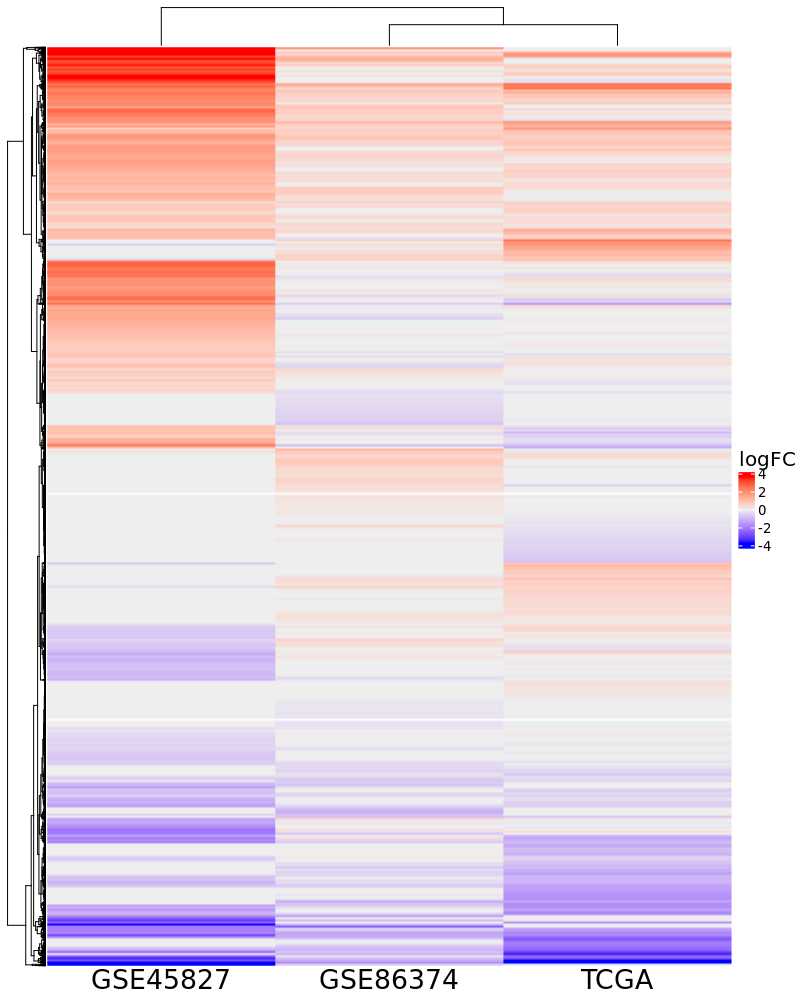
\includegraphics[scale=0.4]{../figures/heatmap.png}
\caption{Valores de expresión diferencial del perfil de expresión del tejido de Luminal A contra tejido sano en cada uno de los sets de datos.}
\label{fig:heatmap}
\end{figure}

Las diferencias en los perfiles de expresión se pueden observar también en la red de co-expresión de Luminal A, previamente calculada, donde se unen las parejas de genes con valores más altos de Información Mutua. La Fig. \ref{fig:networks} muestra más genes sobre-expresados  en el set GSE45827, aunque también se aprecian componentes conexos en la red donde la expresión es similar para los tres data sets.

\begin{figure}
\centering
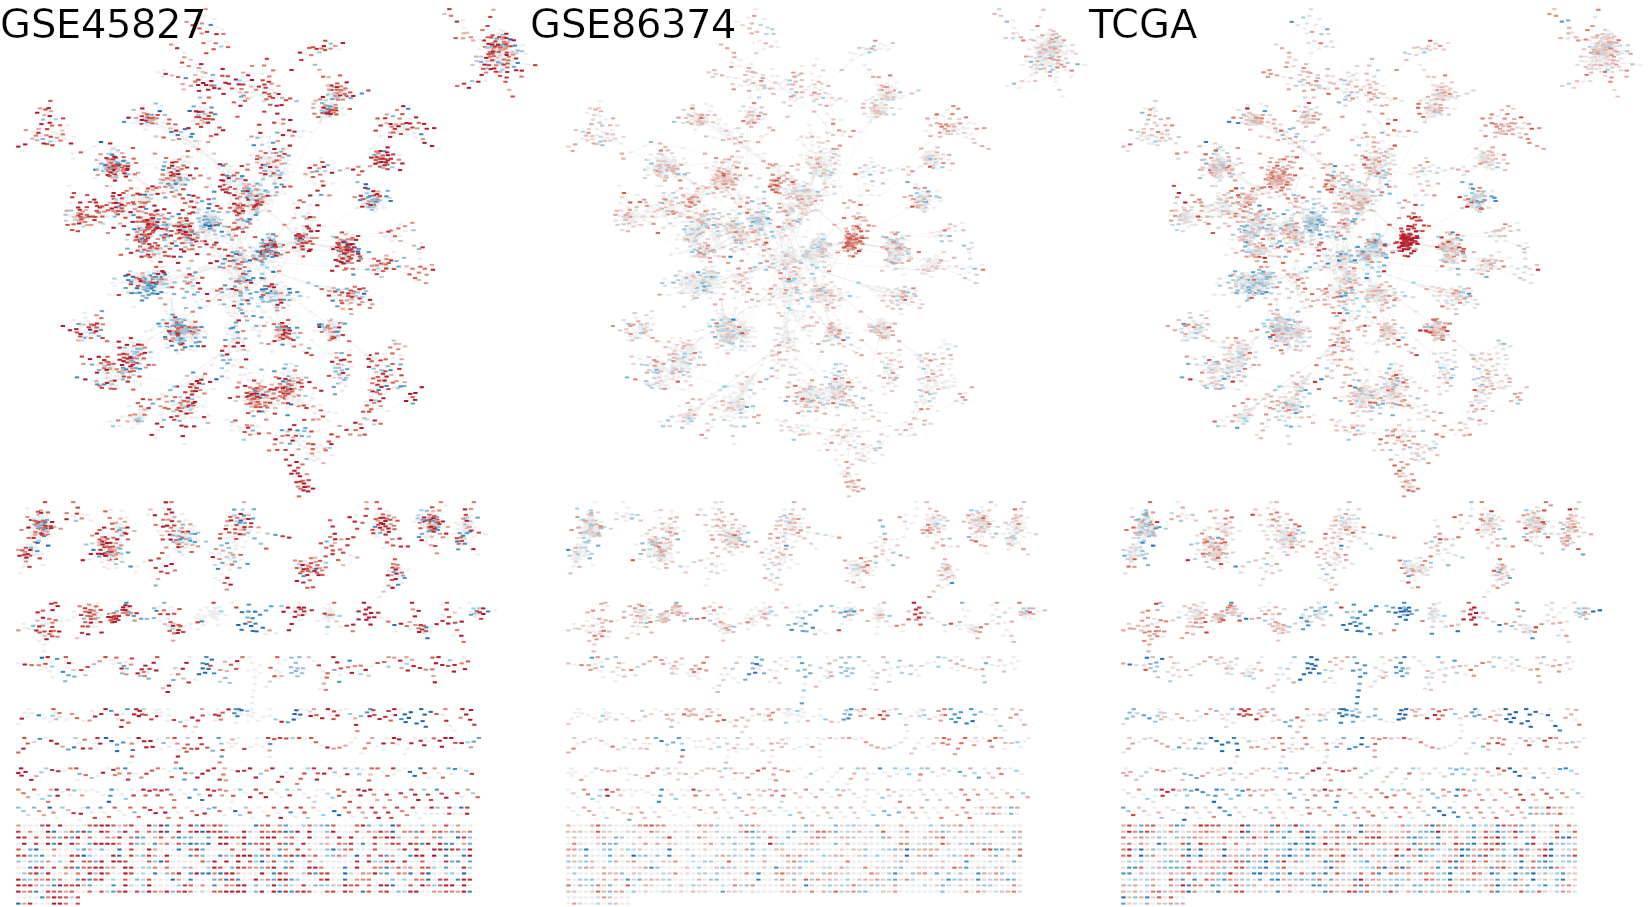
\includegraphics[scale=0.3]{../figures/networks.png}
\caption{Red de valores de co-expresión más altos, calculada con las muestras de TCGA y mostrando los valores de expresión diferencial de cada set de datos.}
\label{fig:networks}
\end{figure}

El número de genes diferencialmente expresados para cada conjunto de datos puede observarse en la Tabla \ref{table:deg}. A pesar de que el número de genes con expresión diferencial es similar para los tres conjuntos, los valores son muy distintos cuando se toman en cuenta cortes de \textit{log fold change}. El data set GSE45827 tiene muchos más genes sobre-expresados, mientras que el set GSE86374 tiene un número muy reducido de gentes tanto sub- como sobre-expresados.

\begin{table}
\centering
\caption{
{Resultado del análisis de expresión diferencial en los conjuntos de datos}}
\begin{tabular}{|l|c|c|c|} 
\hline
 Data set & FDR < 0.5 & FDR < 0.5 y logFC > 2 &  FDR < 0.5 y logFC < 2\\
\hline
\textbf{GSE45827} & 11593 & 1745 & 513  \\
\hline
\textbf{GSE86374} & 11517 & 13 & 32 \\
\hline
\textbf{TCGA} & 12925 & 158 & 560 \\
\hline
\end{tabular}\\
\label{table:deg}
\end{table}

\subsection*{Intersección de procesos biológicos de Gene Ontology enriquecidos en genes con expresión diferencial}

\begin{wrapfigure}{r}{0.4\textwidth}
\centering
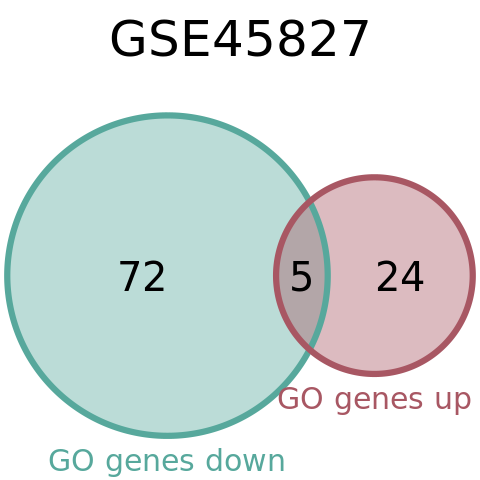
\includegraphics[scale=1.0]{../figures/GSE45827_webgestalt.png}
\caption{Diagrama de Venn de procesos enriquecidos en el set GSE45827}
\label{fig:vennGSE45827}
\end{wrapfigure}

El análisis de WebGestalt para el set de datos GSE86374 obtuvo solamente 4 procesos enriquecidos con FDR < 0.05 para genes sobre-expresados con logFC > 2 y ninguno para genes con logFC < -2, por lo que no fueron tomados en cuenta sus resultados. \\
Para el set GSE45827 se indentificaron 29 procesos enriquecidos en los genes sobre-expresados destancando: la vía de señalización de ERBB, proceso apoptótico en células epiteliales, señalización de Ras y respuestas a TGF$\beta$ y FGF. En los 77 procesos asociados a los genes sub-expresados, encontramos: angiogénesis, proliferación en células epiteliales, regulación de la respuesta a estímulos de factores de crecimiento y diversos procesos relacionados con el metabolismo de lípidos. La Fig. \ref{fig:vennGSE45827} muestra el empalme entre los procesos enriquecidos. \\

\begin{wrapfigure}{l}{0.4\textwidth}
\centering
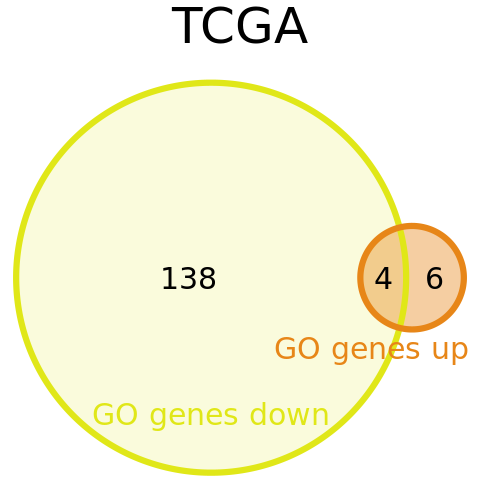
\includegraphics[scale=1.0]{../figures/TCGA_webgestalt.png}
\caption{Diagrama de Venn de procesos enriquecidos en el set de TCGA}
\label{fig:vennTCGA}
\end{wrapfigure}
Para el set de TCGA en los genes sobre-expresados se encontraron 10 procesos enriquecidos. Entre ellos se encuentran segregación de cromosomas y procesos metabólicos relacionados con colágena. En los genes sub-expresados se asociaron 142 procesos, tales como: angiogénesis, proliferación de células epiteliales, regulación positiva de movilidad celular y procesos relacionados con transporte de diferentes metabolitos. \\
El diagrama de venn en la Fig. \ref{fig:venn} del resultado de estos cuatro análisis muestra una mayor intersección en los procesos enriquecidos para los genes sub-expresados. El único proceso biológico enriquecido que se encuentra en los 4 conjuntos es: organización estructural extracelular.\\

\begin{figure}[ht!]
\centering
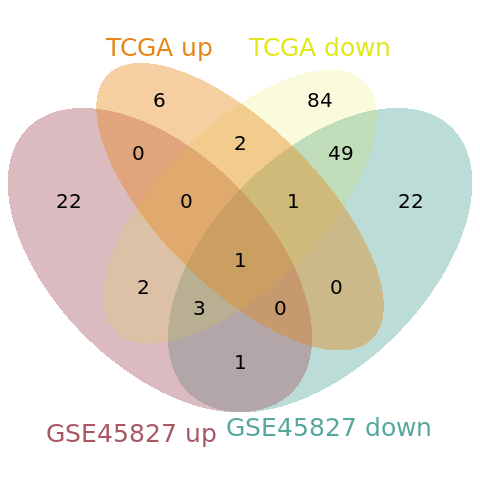
\includegraphics[scale=1.8]{../figures/all_venn.png}
\caption{Diagrama de Venn de procesos enriquecidos en el set de TCGA y el set GSE86374}
\label{fig:venn}
\end{figure}


\subsection*{Resultados del análisis con GSEA}
En el caso del análisis de GSEA en el set GSE45827, a pesar de haber encontrado 2430 sobre-expresados, no se identificó ningún proceso significativo. En el set GSE86374 se encontraron 1486 genes sobre-expresados y solo 6 procesos enriquecidos con FDR < 0.25, sin ser alguno representativo del fenotipo. Para el set de TCGA se encontraron 1125 sobre-expresados y fueron asociados 165 procesos. 

\begin{figure}[ht!]
\centering
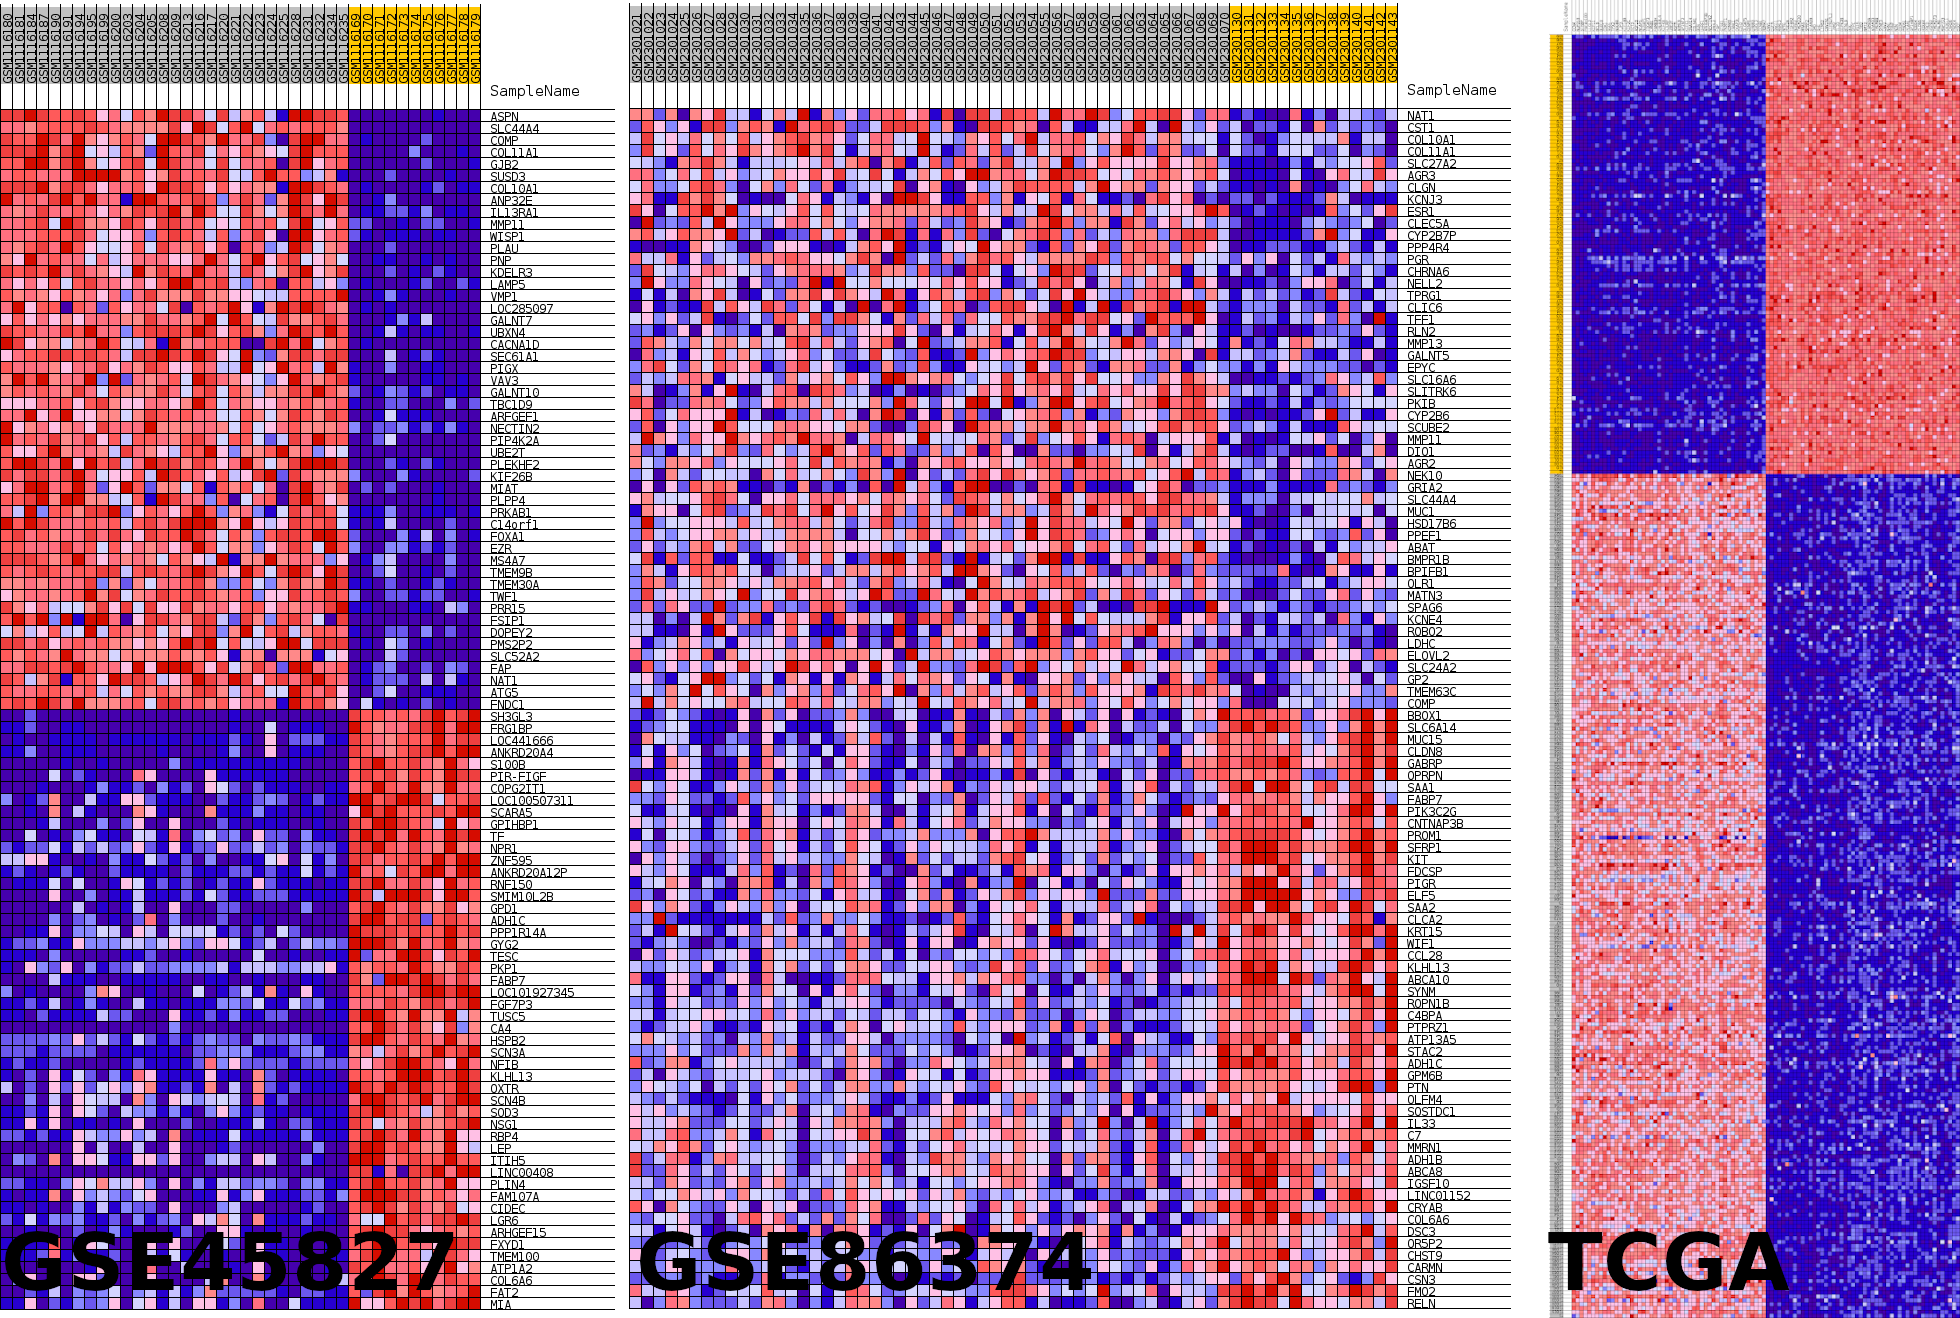
\includegraphics[scale=0.23]{../figures/heatmaps_gsea.png}
\caption{Heatmaps generados por la herramienta GSEA. El heatmap de TCGA está rotado 90 grados en contra de las manecillas del reloj, debido al número de muestras.}
\label{fig:gseah}
\end{figure}

Los heatmaps generados por GSEA que se muestran en la Fig. \ref{fig:gseah} son considerablemente diferentes. Para el set GSE45827 se observa mayor cantidad de genes sobre-expresados. En cambio, en el set de TCGA la cantidad se muestra más balanceada entre genes sobre- y sub- expresados. El set GSE86374 muestra mucha mayor variabilidad entre la expresión de sus genes, al grado de que es difícil reconocer el agrupamiento entre genes sub- y sobre- expresados en las muestras de tejido tumoral y las muestras sanas. \\

\begin{figure}[ht!]
\centering
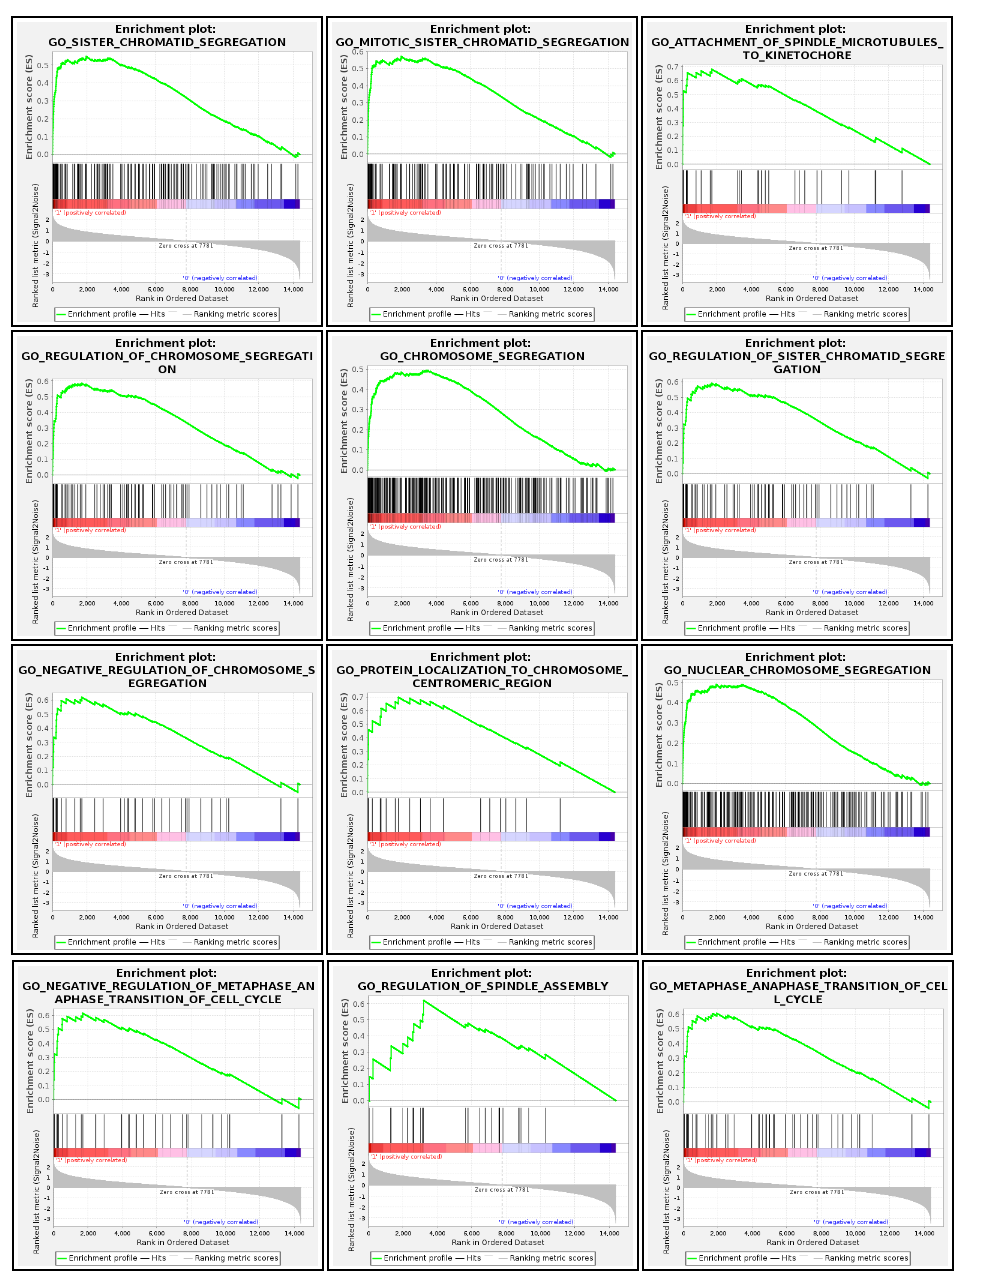
\includegraphics[scale=0.5]{../figures/TCGA_gsea.png}
\caption{Gráficas del score de enriquecimiento para algunos procesos del set de TCGA}
\label{fig:tcgagsea}
\end{figure}

Algunos de los procesos significativos para el set de TCGA se muestran en la Fig. \ref{fig:tcgagsea}. Como puede observarse estos procesos están relacionados con organización y segregación de los cromosomas principalmente durante la división celular. Esto es interesante ya que podría relacionarse con la alta co-expresión en genes dentro del mismo cromosoma, fenómeno que, como se mencionó en la introducción, se observa en todos los subtipos de cáncer de mama. Otros procesos interesantes asociados también de forma significativa son: procesos relacionados con la reparación del ADN, alteración en las marcas de histonas, organización del citoesqueleto, regulación del ciclo celular y mantenimiento de los telómeros. 



\section*{Conclusiones}
En este trabajo se presentaron resultados de la asociación funcional mediante el análisis con WebGestalt y GSEA de tres conjuntos de datos asociados al subtipo Luminal A en cáncer de mama. \\
El set de datos GSE86374 no pudo ser asociado con procesos biológicos de Gene Ontology y sus resultados en GSEA presentaron alta variación en las muestras. Esto podría deberse a que se requieren pasos adicionales en la normalización de los valores de expresión de este set. Por ahora no conocemos el pipeline utilizado para la normalización y procesamiento de estos datos. \\
Los conjuntos de datos de GEO fueron mapeados de identificadores de Entrez a Ensembl para compararlos con el de TCGA en cuanto a niveles de expresión y enriquecimiento con WebGestalt. Así mismo, el conjunto de TCGA se mapeó de Ensembl a símbolos para el análisis de GSEA. Estos mapeos introducen ruido en el análisis ya que no hay una asociación de 1 a 1 entre identificadores y nombres de genes. Además, a pesar de que todos los análisis de expresión se realizaron con el paquete \texttt{limma}, el pre-procesamiento y normalización de los sets de datos es diferente. Finalmente, los conjuntos tienen números distintos de muestras, lo cual puede afectar también los resultados. \\
Sin embargo, aunque existen diversas fuentes de ruido, hay similitudes entre los perfiles de expresión y los procesos enriquecidos, en particular en procesos importantes para el cáncer como la angiogénesis, proliferación celular, regulación del ciclo celular y mantenimiento de telómeros, demostrando la utilidad de las herramientas computacionales en el análisis de los perfiles de expresión y su asociación a características funcionales. 

\bibliographystyle{vancouver} % Style BST file (bmc-mathphys, vancouver, spbasic).
%\bibliography{gcdd}      % Bibliography file (usually '*.bib' @article {Garc{\'\i}a-Cort{\'e}s399253,

\begin{thebibliography}{1}

\bibitem{gdc} Garc{\'\i}a-Cort{\'e}s, Diana and de Anda-J{\'a}uregui, Guillermo and Fresno, Crist{\'o}bal and Hernandez-Lemus, Enrique and Espinal-Enr{\'\i}quez, Jes{\'u}s. {\em Gene co-expression is distance-dependent in breast cancer.} bioRxiv, 2020.
\bibitem{GSE86374} Analysis of somatic DNA copy number alterations and frequency of breast cancer intrinsic subtypes from Mexican women [gene expression]. \url{https://www.ncbi.nlm.nih.gov/geo/query/acc.cgi?acc=GSE86374}, 2018.
\bibitem{GSE45827} Expression data from Breast cancer subtypes \url{https://www.ncbi.nlm.nih.gov/geo/query/acc.cgi?acc=GSE45827}, 2016.
\end{thebibliography}


\end{document}
